%%%%%%%%%%%%%%%%%%%%%%%%%%%%%%%%%%%%%%%%%
% Short Sectioned Assignment LaTeX Template Version 1.0 (5/5/12)
% This template has been downloaded from: http://www.LaTeXTemplates.com
% Original author:  Frits Wenneker (http://www.howtotex.com)
% License: CC BY-NC-SA 3.0 (http://creativecommons.org/licenses/by-nc-sa/3.0/)
%%%%%%%%%%%%%%%%%%%%%%%%%%%%%%%%%%%%%%%%%

%----------------------------------------------------------------------------------------
%	PACKAGES AND OTHER DOCUMENT CONFIGURATIONS
%----------------------------------------------------------------------------------------

\documentclass[paper=a4, fontsize=11pt]{scrartcl} % A4 paper and 11pt font size

% ---- Entrada y salida de texto -----

\usepackage[T1]{fontenc} % Use 8-bit encoding that has 256 glyphs
\usepackage[utf8]{inputenc}
%\usepackage{fourier} % Use the Adobe Utopia font for the document - comment this line to return to the LaTeX default

% ---- Idioma --------

\usepackage[spanish, es-tabla]{babel} % Selecciona el español para palabras introducidas automáticamente, p.ej. "septiembre" en la fecha y especifica que se use la palabra Tabla en vez de Cuadro

% ---- Otros paquetes ----

\usepackage{url} % ,href} %para incluir URLs e hipervínculos dentro del texto (aunque hay que instalar href)
\usepackage{amsmath,amsfonts,amsthm} % Math packages
%\usepackage{graphics,graphicx, floatrow} %para incluir imágenes y notas en las imágenes
\usepackage{graphics,graphicx, float} %para incluir imágenes y colocarlas

\usepackage{enumitem}

% Para hacer tablas comlejas
%\usepackage{multirow}
%\usepackage{threeparttable}

% Para utilizar pseudocódigo
\usepackage{algorithm}
\usepackage{algorithmic}
\usepackage{algorithmicx}
\usepackage{listings}

%\usepackage{sectsty} % Allows customizing section commands
%\allsectionsfont{\centering \normalfont\scshape} % Make all sections centered, the default font and small caps

\usepackage{fancyhdr} % Custom headers and footers
\pagestyle{fancyplain} % Makes all pages in the document conform to the custom headers and footers
\fancyhead{} % No page header - if you want one, create it in the same way as the footers below
\fancyfoot[L]{} % Empty left footer
\fancyfoot[C]{} % Empty center footer
\fancyfoot[R]{\thepage} % Page numbering for right footer
\renewcommand{\headrulewidth}{0pt} % Remove header underlines
\renewcommand{\footrulewidth}{0pt} % Remove footer underlines
\setlength{\headheight}{13.6pt} % Customize the height of the header

\numberwithin{equation}{section} % Number equations within sections (i.e. 1.1, 1.2, 2.1, 2.2 instead of 1, 2, 3, 4)
\numberwithin{figure}{section} % Number figures within sections (i.e. 1.1, 1.2, 2.1, 2.2 instead of 1, 2, 3, 4)
\numberwithin{table}{section} % Number tables within sections (i.e. 1.1, 1.2, 2.1, 2.2 instead of 1, 2, 3, 4)

\setlength\parindent{0pt} % Removes all indentation from paragraphs - comment this line for an assignment with lots of text

\newcommand{\horrule}[1]{\rule{\linewidth}{#1}} % Create horizontal rule command with 1 argument of height


%----------------------------------------------------------------------------------------
%	TÍTULO Y DATOS DEL ALUMNO
%----------------------------------------------------------------------------------------

\title{	
\normalfont \normalsize 
\textsc{\textbf{Metaheurística} \\ Doble Grado en Ingeniería Informática y Matemáticas \\ Universidad de Granada} \\ [25pt] % Your university, school and/or department name(s)
\horrule{0.5pt} \\[0.4cm] % Thin top horizontal rule
\Huge Práctica 1\\
\LARGE Algorítmos basados en trayectorias en Problema de Asignación Cuadrática(QAP)
 \\ % The assignment title
\horrule{2pt} \\[0.5cm] % Thick bottom horizontal rule
}

\author{ Iván Sevillano García \\\\
	DNI: 77187364-P\\ \\
	E-mail: ivansevillanogarcia@correo.ugr.es\\\\
	Grupo del martes, 17:30h-19:30h
	} % Nombre y apellidos

\date{\normalsize\today} % Incluye la fecha actual

%----------------------------------------------------------------------------------------
% DOCUMENTO
%----------------------------------------------------------------------------------------

\begin{document}

\maketitle % Muestra el Título

\newpage

\tableofcontents
\newpage

\section{Descripción del problema QAP}

El problema que se nos plantea es el Problema de Asignación Cuadrática(en adelante QAP por las siglas). En él, tenemos una serie de instalaciones las cuales tienen que interactuar entre ellas una cierta "cantidad de trabajo", produciendo un coste. Las instalaciones tienen, además, unas determinadas localizaciones en las que se tienen que situar. Dependiendo de la distancia entre cada dos instalaciones, el coste que producen al interactuar es mayor o menor.\\

Cabe destacar una serie de detalles en el problema:

\begin{itemize}
	\item \textbf{No Euclideo(No Métrico).} Este problema  no pone ninguna objeción a que la distancia de una localización de un lugar a si mismo sea mayor que cero. Además, una instalación puede interactuar consigo misma por consiguiente.
	\item \textbf{No simétrico.} Tampoco pone objeción a que la distancia de una localización a otra no sea la misma que de otra a una.
\end{itemize}

El problema entonces consiste en repartir las instalaciones en las localizaciones de forma que el coste total o trabajo sea mínimo. Esto es fácil de representar con una permutación, que a cada instalación $i$ le asigna una localización $\pi(i)$. Si llamamos $d_{ij}$ a la distancia que hay de la localización $i$ a la $j$, y $f_{ij}$ la cantidad de trabajo que tiene que mandar la instalación $i$ a la $j$, la función de coste asociada al problema sería la siguiente:

\[Coste(\pi)=\sum_{i=1}^{N}\sum_{j=1}^{N}f_{ij}d_{\pi(i)\pi(j)}\]

Si consideramos las matrices de distancias y flujos, $D$ y $F$ y las matrices de que representan a cada permutación y su inversa, $\Pi$ y $\Pi^{-1}$ respectivamente, se puede representar el coste de una manera más sencilla:

\[Coste(\pi)=<F,\Pi^{-1}D\Pi> \]

Donde la aplicación $<,>$ tiene como argumentos dos matrices de mismas dimensiones y se aplica en la suma de la multiplicación de sus componentes una a una. 

\newpage

\section{Breve descripción de los algorítmos utilizados.}
En esta sección vamos a explicar brevemente la configuración de una solución concreta del problema, el funcionamiento de la función de coste y de cómo trabajan los dos algoritmos que se describen en el enunciado.

\subsection{Solución.}

Una solución está perfectamente determinada por un vector de $N$ componentes donde cada una de sus componentes es distinta unas de otras y el rango de valores difiere de 1 hasta N, o lo que es lo mismo, la solución es una permutación. Según la misma, la localización $i$ tendrá alojada la instalación con el número que ocupa en el vector la posición $i$. Para agilizar cálculos, cada permutación, además, guarda su coste asociado. Así, será fácil calcular soluciones vecinas.

\subsection{Función de coste.}

La función de coste es la descrita anteriormente en la primera sección. A continuación el psudo-código. Los parámetros hacen referencia a la matriz de distancias(D), la matriz de flujos(F) y a la permutación que representa nuestra solución:\\

\begin{lstlisting}
Parametros:D,F,P
Output: coste
coste = 0
Para cada elemento de la matriz (i,j):
  coste <- coste + F[j][i]*D[P(j)][P(i)]
\end{lstlisting}


\subsection{Algoritmos basados en trayectorias.}

Esta práctica consistirá en desarrollar cuatro algoritmos basado en trayectorias y un algoritmo híbrido entre dos de ellos. Veamos ahora las descripciones de cada uno de ellos:\\

\subsubsection{Búsqueda multiarranque básico.}

Este algorítmo consiste en utilizar la ya conocida búsqueda local a partir de varios puntos o soluciones de arranque. Puesto que  condición de parada son las mismas evaluaciones, se realizarán menos evaluaciones en cada una de las búsquedas locales del algoritmo. 

\subsubsection{Enfriamiento simulado(ES).}

Este algoritmo se basa en cómo  se comportan una partícula dentro de un metal al enfriarse el mismo. Al principio, esta partícula tiene mucha energía por la alta temperatura, por lo que se mueve mucho aunque vaya a posiciones con más "energía". Conforme se va enfriando el metal, lo mismo le pasa a la partícula y tiene menos energía, por lo que los saltos que hace se empiezan a parecer más a una búsqueda por descenso, intentando ir a posiciones con cada vez menos energía. Pasamos a describir cada una de las características:

\begin{itemize}
	\item \textbf{Aceptación de soluciones.} Este algoritmo se basa en poder aceptar soluciones de peor calidad dependiendo de la temeratura actual. Así, una solución será aceptada cuando:\\
	
	\begin{itemize}
		\item La solución S' es mejor que la solución S actual con una probabilidad de 1.
		\item La solución S' es peor que la solución S actual con una probabilidad de $ e^{\dfrac{-dC}{T_i}}$, donde $dC$ es la diferencia de coste entre la solución actual S y S'. $dC$ es un número positivo ya que S' no mejora a la solución actual. $T_i$ es la temperatura actual. Por tanto, la expresión antes descrita es un número entre 0 y 1 que podremos usar como probabilidad. Además se pueden hacer varias observaciones.\\
		
		La primera es que si la temperatura es muy alta la probabilidad con la que vamos a aceptar una solución es prácticamente 1. Si es muy baja, es casi 0. \\
		
		La segunda, que conforme va avanzando el algoritmo, $dC$ empieza a tener más importancia. Tanto cuando la temperatura es muy alta como cuando es muy baja, $dC$ no afecta demasiado a la aceptación de la solución. Sin embargo, en mitad de la ejecución si es más relevante. Se aceptarán soluciones dependiendo de cuanta diferencia de coste hay entre soluciones.
	
	\end{itemize}
	\item \textbf{Esquema de enfriamiento.} En cada etapa del algoritmo modificaremos la temperatura de la siguiente manera:
	
	\[T_{k+1}=\dfrac{T_k}{1+\beta T_{k}},\beta = \dfrac{T_0-T_f}{MT_0T_f} \]
	 
	 Donde M es el número de enfriamientos. Este es distinto a número de evaluaciones de la función objetivo. Se harán, dentro de una misma etapa de enfriamiento, varias evaluaciones de la función objetivo.
	 
	 \item \textbf{Operador de vecino.} Se utiliza el mismo operador de vecino que en la búsqueda local de la primera práctica. En cada iteración se explorará sólo un vecino que pueda sustituir a la solución actual.
	 
	 \item \textbf{Condición de enfriamiento.} La condición que se quiere considerar en la práctica para enfriar es haber alcanzado un máximo de evaluaciones de nuevos vecinos o haber alcanzado un máximo de vecinos aceptados.
	 
	 \item \textbf{Condición de parada.} El algoritmo finalizará si se llega al máximo de evaluaciones o si en la iteración actual no ha encontrado ninguna solución que hayamos aceptado. Esta última consideración se impone en la práctica pero veremos que pasa si la suprimimos.
	
	
\end{itemize}

Los valores de los parámetros escogidos en esta práctica son los siguientes:\\

\[T_0=\dfrac{\mu C(S_0)}{-ln(\phi)},T_f=10^{-3},\mu=\phi=0.3\]

Se debe comprobar que la temperatura final es menor que la inicial. Como número máximo de vecinos en cada enfriamiento se ha escogido 10 veces el tamaño del problema. Como número de éxitos, la décima parte de este número. Así, el número de enfriamientos será $50000/max\_vecinos$.



\subsubsection{Búsqueda local iterativa(ILS).}

En este algoritmo ejecutaremos de forma repetida una búsqueda local. Cada cierto tiempo, modificaremos una parte significativa de la solución generando una solución vecina más lejana a la vecina de la búsqueda local, y volveremos a aplicar sobre esta nueva solución la búsqueda local. 

\subsubsection{Búsqueda por procedimiento greedy aleatorizado(GRASP).}


\subsubsection{Algoritmo híbrido. ILS-ES}

\newpage
\section{Pseudocódigos y explicaciones.}

A continuación se detallan los pseudocódigos de los algoritmos immplementados:\\

\subsection{AG generacional.}

\begin{lstlisting}
Pobl = 50 soluciones aleatorias.
Hasta que se superen las 50.000 evaluaciones:
  Selecciona por torneoBinario 50 padres(copias).
  Sustituye el primer 70% por los hijos generados al cruzar cada 2.
  
  Para cada mutacion que debamos hacer en H hijo, (i,j):
    Sustituimos H por su vecino (i,j)
  Si la nueva poblacion no mejora a la mejor solucion
  anterior:
    Se sustituye la peor solucion por la mejor solucion de la
    poblacion anterior.
  
  Se sustituye la poblacion anterior por la actual.
\end{lstlisting}

\subsection{AG estacionario.}

\begin{lstlisting}
Pobl = 50 soluciones aleatorias.
Hasta que se superen las 50.000 evaluaciones:
  Selecciona por torneoBinario 2 padres(copias).
  Genera dos hijos con los cruces seleccionados.

  Para cada mutacion que debamos hacer en H hijo, (i,j):
    Sustituimos H por su vecino (i,j)

  Sacamos de la poblacion anterior a las dos peores soluciones.

  Introducimos en la poblacion a las dos soluciones con
  mejor coste de entre las dos peores y los dos hijos.
\end{lstlisting}

\subsection{Algoritmos meméticos}

Las posibles mejoras meméticas se pueden modelizar con dos variables: la proporción de la población a la que se le va a aplicar la búsqueda local y si esa proporción va a ser la de los mejores:

\begin{lstlisting}
Input: Pobl, p_pobl,mejores

Si se escogen los mejores:
  Se ordena el vector de poblacion por coste ascendente.
Si no y p_pobl < 1:
  Se mezcla el vector Pobl.

Se aplica la busqueda local con un tope de 400 pasos a las primeras
soluciones de la poblacion(Cantidad proporcional a p_pobl).
\end{lstlisting}

\newpage

\subsection{Consideraciones de parada de cada algoritmo.}



\newpage

\section{Algoritmo de comparación.}
En esta sección se compararán los resultados de los algoritmos Greedy y búsqueda local. Para dicha comparación, atenderemos a dos estadísticos:\\

\begin{itemize}
	\item \textbf{Desviación a la solución óptima.} Este estadístico evaluará proporcionalmente la diferencia de coste de la mejor solución y la solución obtenida en cada instancia.La fórmula que describe este estadístico es el siguiente:
	\[Desv = \dfrac{1}{ \left| casos\right|}\sum_{i \in casos}100\dfrac{valorAlg_i - mejorVal_i}{mejorVal_i} \]
	
	\item \textbf{Tiempo medio de ejecución.} La media de los tiempos de ejecución de cada algoritmo.
\end{itemize}

Consideraremos entonces que un algoritmo es mejor que otro si la desviación a la solución óptima es menor. En caso de ser iguales, el algoritmo que tarde menos será considerado mejor.

\newpage

\section{Manual de uso.}

Para la implementación de la práctica hemos utilizado el lenguaje precompilado Python3, por lo que debe de estar instalado en el sistema. También hemos hecho uso de la biblioteca random del mismo lenguaje, más en concreto de las funciones randint(inicio,fin), que escoge aleatoriamente un valor entero entre  $inicio$ y $fin-1$, y shuffle(vector), que mezcla el vector que se le pasa como argumento.\\

La forma de utilizar el programa es la siguiente:\\

\begin{itemize}
	\item \textbf{Programas.} Esta practica tiene un total de siete ejecutables. Cadaejecutable recibe como argumento el nombre del archivo de entrada con los datos(terminado en '.dat'), que debe de estar en el directorio $./qapdata/$. Tiene que haber también un archivo solución con el mismo nombre pero con terminación '.sln'  en el directorio $./qapsoln/$. Es posible también introducir una semilla como segundo argumento y un fichero de salida:\\
	
	$./nombreAlgoritmo.py$ $./qapdata/nombredatos.dat$ $semilla$ $fichero_salida$\\
	
	Nos dará como resultado:\\
	\begin{itemize}
		\item Solución Algoritmo. La primera linea será la solución del algoritmo en cuestión obtenida. La segunda, cuanto tiempo ha tardado el programa en calcularla y cuanto coste total tiene esta solución.
		\item Mejor solución. La primera linea es la configuración de la mejor solución y la siguiente es su coste.
	\end{itemize}
	
	\item \textbf{Experimento total.} Para ejecutar el experimento completo, nos hemos ayudado de un script que ejecuta todos los casos de prueba y un makefile que lo llama. Así, la forma de obtener todas las soluciones será tan simple como ejecutar el siguiente comando:\\
	
	$make$ $all$\\
	
	Es importante mencionar que dentro de la ejecución de los programas se les ha introducido una semilla en concreto, $200000$, que no modificaremos.\\
	
	
\end{itemize}

\newpage
\section{Experimento y análisis de resultados.}

Las tablas obtenidas para cada algoritmo son las siguientes:\\


\input{./tablasLatex/BMB.txt}


\input{./tablasLatex/ES.txt}


\input{./tablasLatex/ILS.txt}


\input{./tablasLatex/GRASP.txt}


\input{./tablasLatex/ILS-ES.txt}





\newpage
Por último, la tabla de comparación de algoritmos:

\begin{table}[htbp]
	\begin{center}
		\begin{tabular}{|l|l|l|}
			\hline
			Algoritmo &  Desv & Tiempo\\
			\hline \hline
			Greedy& 59.73 & 0,00\\ \hline
			BL & 8.34 & 13.45 \\ \hline
			BMB & 24.98 & 15.9\\ \hline
			ES & 20.98& 19.05\\ \hline
			ILS & 18.06 & 71.62\\ \hline
			GRASP & 8.03 & 70.61\\ \hline
			ILS-ES & 26.72 & 20.59\\ \hline
		\end{tabular}
		\caption{Tabla de comparación}
		\label{tabla:TablaComparacion}
	\end{center}
\end{table}

\subsection{Análisis de resultados}

La primera consideración que hacemos es la comparativa entre los dos cruces que hemos implementado. El primer cruce tiene peores resultados que el PMX. Esto puede darse por la aleatoriedad en el cruce subyacente, que no aprovecha toda la información que podría utilizar de la permutación.\\

Según los estadísticos que hemos recogido queda claro que ningún algoritmo aquí implementado es mejor que la búsqueda local de la práctica anterior. Sin embargo hay algunos casos en los que los algoritmos si se comportan mejor. Un ejemplo de ello es el caso de $chr22a.dat$. Veamos cómo evoluciona en cada generación de cada algoritmo la mejor función de coste.

\begin{figure}[H]
	\centering
	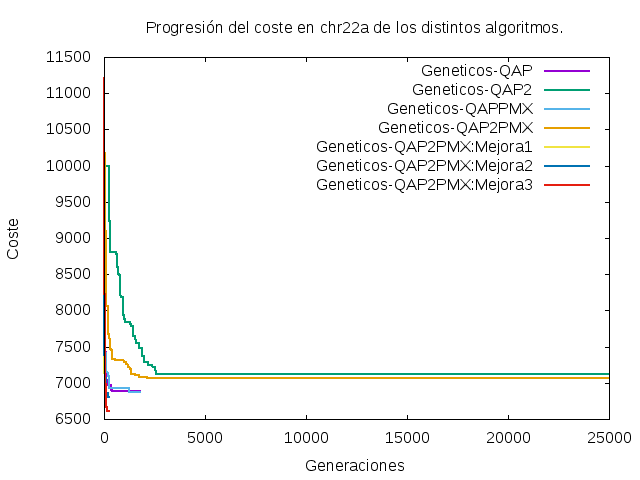
\includegraphics[width=0.7\linewidth]{graficos/comparativachr22a}
	\caption[Comparativa chr22a]{Comparativa chr22a}
	\label{fig:comparativachr22a}
\end{figure}

En este gráfico se ve claramente que se han obtenido muchas generaciones en los algoritmos genéticos estacionarios mientras que tanto los meméticos como los generacionales han utilizado menos generaciones. Sin embargo, ambos han conseguido rebajar mucho más rápido la función de coste, incluso han superado el mínimo local en el que se han quedado estancados los algoritmos estacionarios.\\

Esto no ocurre en otras instancias, como por ejemplo en $sko81$:\\

\begin{figure}[H]
	\centering
	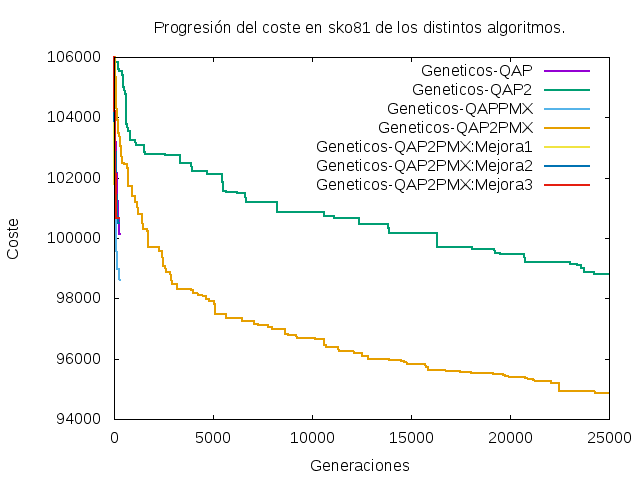
\includegraphics[width=0.7\linewidth]{graficos/comparativasko81}
	\caption[Comparativa sko81]{Comparativa sko81}
	\label{fig:comparativasko81}
\end{figure}

Este gráfico nos muestra que, con las iteraciones máximas que le hemos puesto, los algoritmos tanto meméticos como generacionales no han tenido tiempo de dar una solución de calidad. Sin embargo, los algoritmos estacionarios si han podido ir mejorando su coste de forma progresiva. En los siguientes dos casos se tienen comportamientos similares, solo que en la pocas iteraciones si que se ha conseguido un coste parecido:\\

\begin{figure}[H]
	\centering
	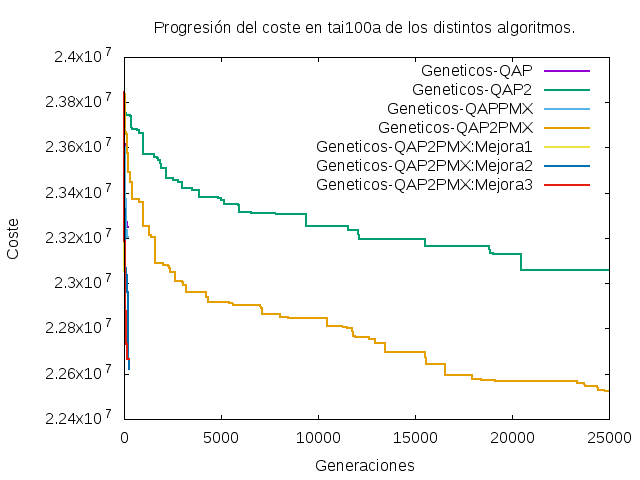
\includegraphics[width=0.7\linewidth]{graficos/comparativatai100a}
	\caption[Comparativa tai100a]{Comparativa tai100a}
	\label{fig:comparativatai100a}
\end{figure}

\begin{figure}[H]
	\centering
	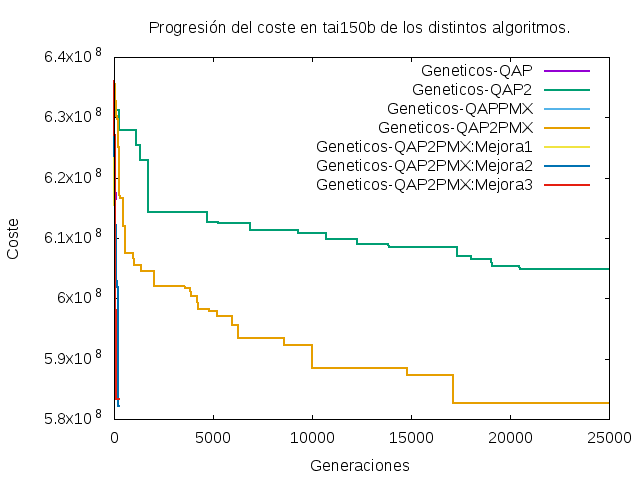
\includegraphics[width=0.7\linewidth]{graficos/comparativatai150b}
	\caption[Comparativa tai150b]{Comparativa tai150b}
	\label{fig:comparativatai150b}
\end{figure}

Por último, en la instancia más grande(tai256c) no se consigue apenas una mejora consistente, volvemos al caso de  sko81:\\

\begin{figure}[H]
\centering
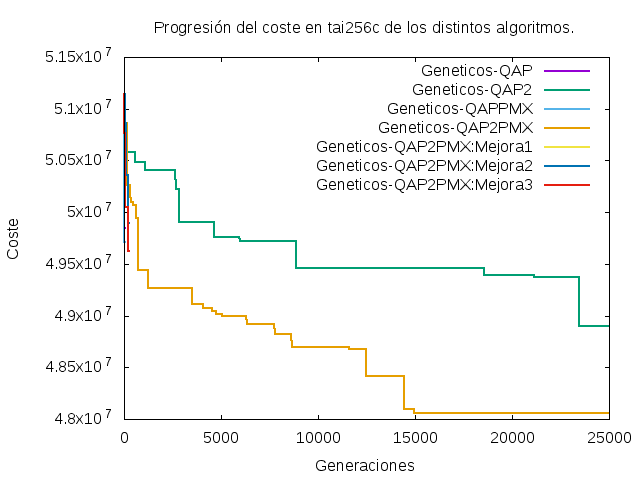
\includegraphics[width=0.7\linewidth]{graficos/comparativatai256c}
\caption[]{Comparativa 256c}
\label{fig:comparativatai256c}
\end{figure}

\subsection{Análisis de AG generacionales.}

En las gráficas antes vistas se puede observar fácilmente el comportamiento de los algoritmos estacionarios ya que tienen muchas generaciones. Veamos ahora el comportamiento en concreto de los algoritmos generacionales y meméticos:

\begin{figure}[H]
\centering
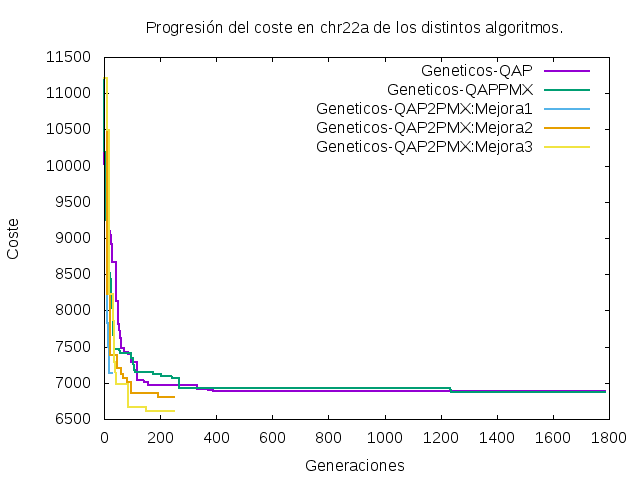
\includegraphics[width=0.7\linewidth]{graficos/comparativaGeneracionalchr22a}
\caption{Comparativa generacional vs meméticos estacionarios chr22a}
\label{fig:comparativaGeneracionalchr22a}
\end{figure}

Lo primero que notamos en esta comparativa es que, aun evaluando muchísimas veces la función objetivo en cada generación de los algoritmos genéticos generacionales, en un problema de tamaño pequeño los algoritmos meméticos utilizan muy pocas generaciones en comparación. Esto se debe a la cantidad de mutaciones que hacemos. Veamos que ocurre en las siguientes instancias:\\

\begin{figure}[H]
\centering
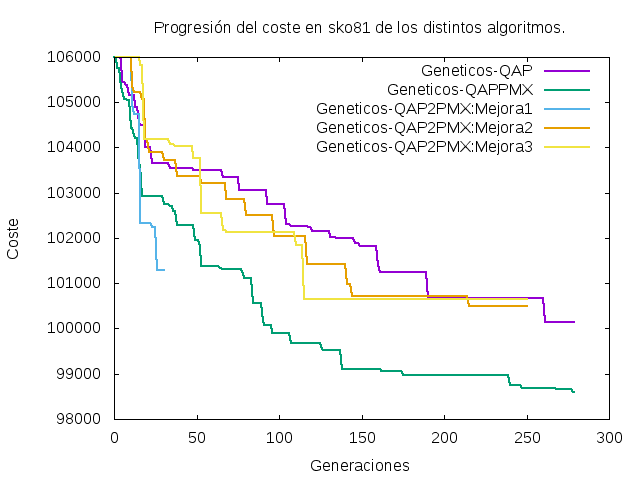
\includegraphics[width=0.7\linewidth]{graficos/comparativaGeneracionalsko81}
\caption{Comparativa generacional vs meméticos estacionarios sko81}
\label{fig:comparativaGeneracionalsko81}
\end{figure}

En esta instancia el número de generaciones se igualan ya que se evalúa más veces la función objetivo gracias a las mutaciones. También se puede observar que la evolución de los algoritmos meméticos se produce a saltos. Otro dato importante a tener en cuenta es que, pese a tener mejor estadístico la tercera mejora,  en esta instancia la segunda mejora lo supera. La primera mejora tiene muchas menos iteraciones ya que utiliza la mayoría de las evaluaciones de la función coste en búsquedas locales.\\

En los siguientes gráficos se ve cómo decrece el número de generaciones de los algoritmos genéticos generacionales mientras que los meméticos estacionarios mantienen sus generaciones fijas:\\

\begin{figure}[H]
	\centering
	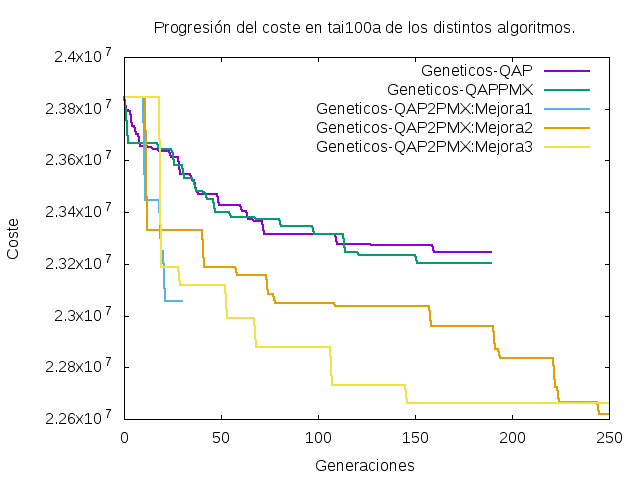
\includegraphics[width=0.7\linewidth]{graficos/comparativaGeneracionaltai100a}
	\caption{Comparativa generacional vs meméticos estacionarios tai100a}
	\label{fig:comparativaGeneracionaltai100a}
\end{figure}
 
\begin{figure}[H]
\centering
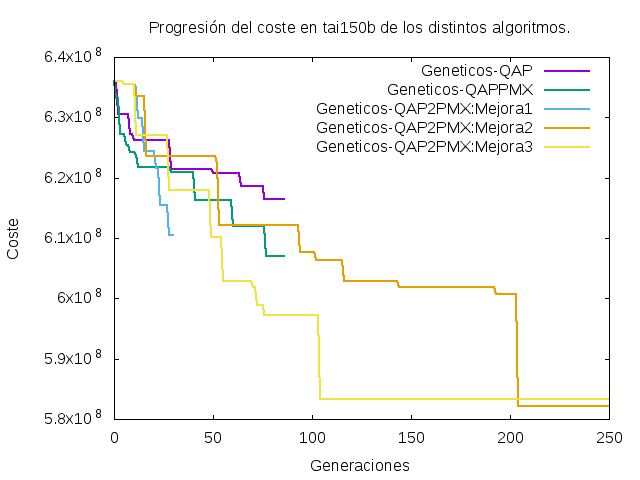
\includegraphics[width=0.7\linewidth]{graficos/comparativaGeneracionaltai150b}
\caption{Comparativa generacional vs meméticos estacionarios tai150b}
\label{fig:comparativaGeneracionaltai150b}
\end{figure}

\begin{figure}[H]
\centering
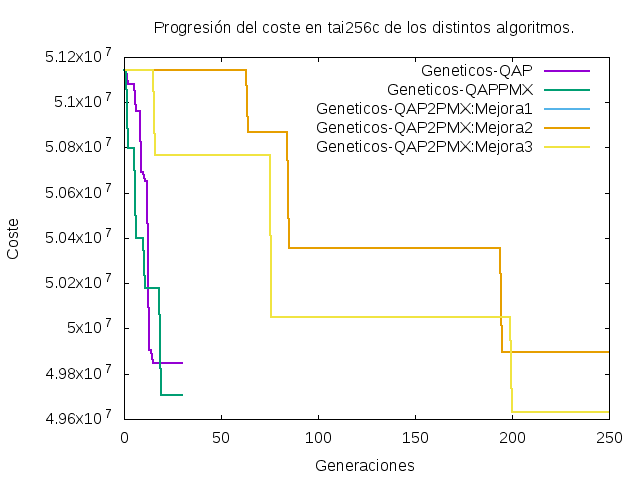
\includegraphics[width=0.7\linewidth]{graficos/comparativaGeneracionaltai256c}
\caption{Comparativa generacional vs meméticos estacionarios tai256c}
\label{fig:comparativaGeneracionaltai256c}
\end{figure}

\subsection{Posibles mejoras de los algoritmos}

Como ya se dijo en el apartado de consideraciones de parada, hay varias ideas en los algoritmos que se deben pulir:\\

\begin{itemize}
	\item \textbf{Tiempo de ejecución.} Las mutaciones, aunque sean evaluaciones de la función objetivo, tardan mucho menos en ser evaluadas. Se debería poder evaluar muchas veces tales mutaciones sin que ello repercutiese demasiado en el número de evaluaciones totales.
	
	\item \textbf{Evaluaciones por BL}. En los algoritmos meméticos la búsqueda local solo dispone de 400 evaluaciones. Si consideramos los primeros 400 genes, nunca se podrá mejorar los últimos. Para poder solventar esto, se podría empezar a profundizar en cada búsqueda local en un gen distinto o incluso aleatorizar la selección del gen a investigar. Otra forma de poder mejorar este aspecto es que el número de evaluaciones de la búsqueda local asegurase que intenta cambiar y mejorar al menos una vez cada gen. Es decir, que en vez de tener un número fijo de evaluaciones(400), este número dependa del número de genes(posibles trasposiciones $(i,j)$).
	
	\item \textbf{Parámetros modificables.} Dependiendo del tamaño del problema podríamos modificar cada cuanto se debe realizar una búsqueda local en los algoritmos meméticos, ya que estos consumen muchas evaluaciones y no dejan al algoritmo genético evolucionar para producir diversidad. De hecho, la última mejora se podría considerar que se comporta casi como una búsqueda local multiarranque en algunos casos(aplicando siempre la búsqueda local a los mejores).
	
\end{itemize}








\end{document}





